\documentclass[11pt,a4paper,onecolumn]{IEEEtran}
\usepackage[margin=3cm]{geometry}
\usepackage[english]{babel}
\usepackage{graphicx}
\usepackage{lipsum}
% Path relative to the .tex file containing the \includegraphics command
\graphicspath{ {./images/} }

\title{Promsie Javascript\\
{\footnotesize RWTH Aachen University}}

\author{
  \IEEEauthorblockN{1\textsuperscript{st} Papop Lekhapanyaporn}
  \and
  \IEEEauthorblockN{2\textsuperscript{nd} Tobias Piatek}
  \and
  \IEEEauthorblockN{3\textsuperscript{rd} Tobias Waerder}
  }



\begin{document}
\maketitle
\begin{abstract}
  \lipsum[1]
\end{abstract}
\section{Promises}
\lipsum[2]
\subsection{then}
\lipsum[3]
\subsection{catch}
\lipsum[4]
\section{Asynchronous methods}
\lipsum[4-6]
\subsection{async}
\lipsum[3]
\subsection{await}
\lipsum[4]
\begin{figure}
  \centering
  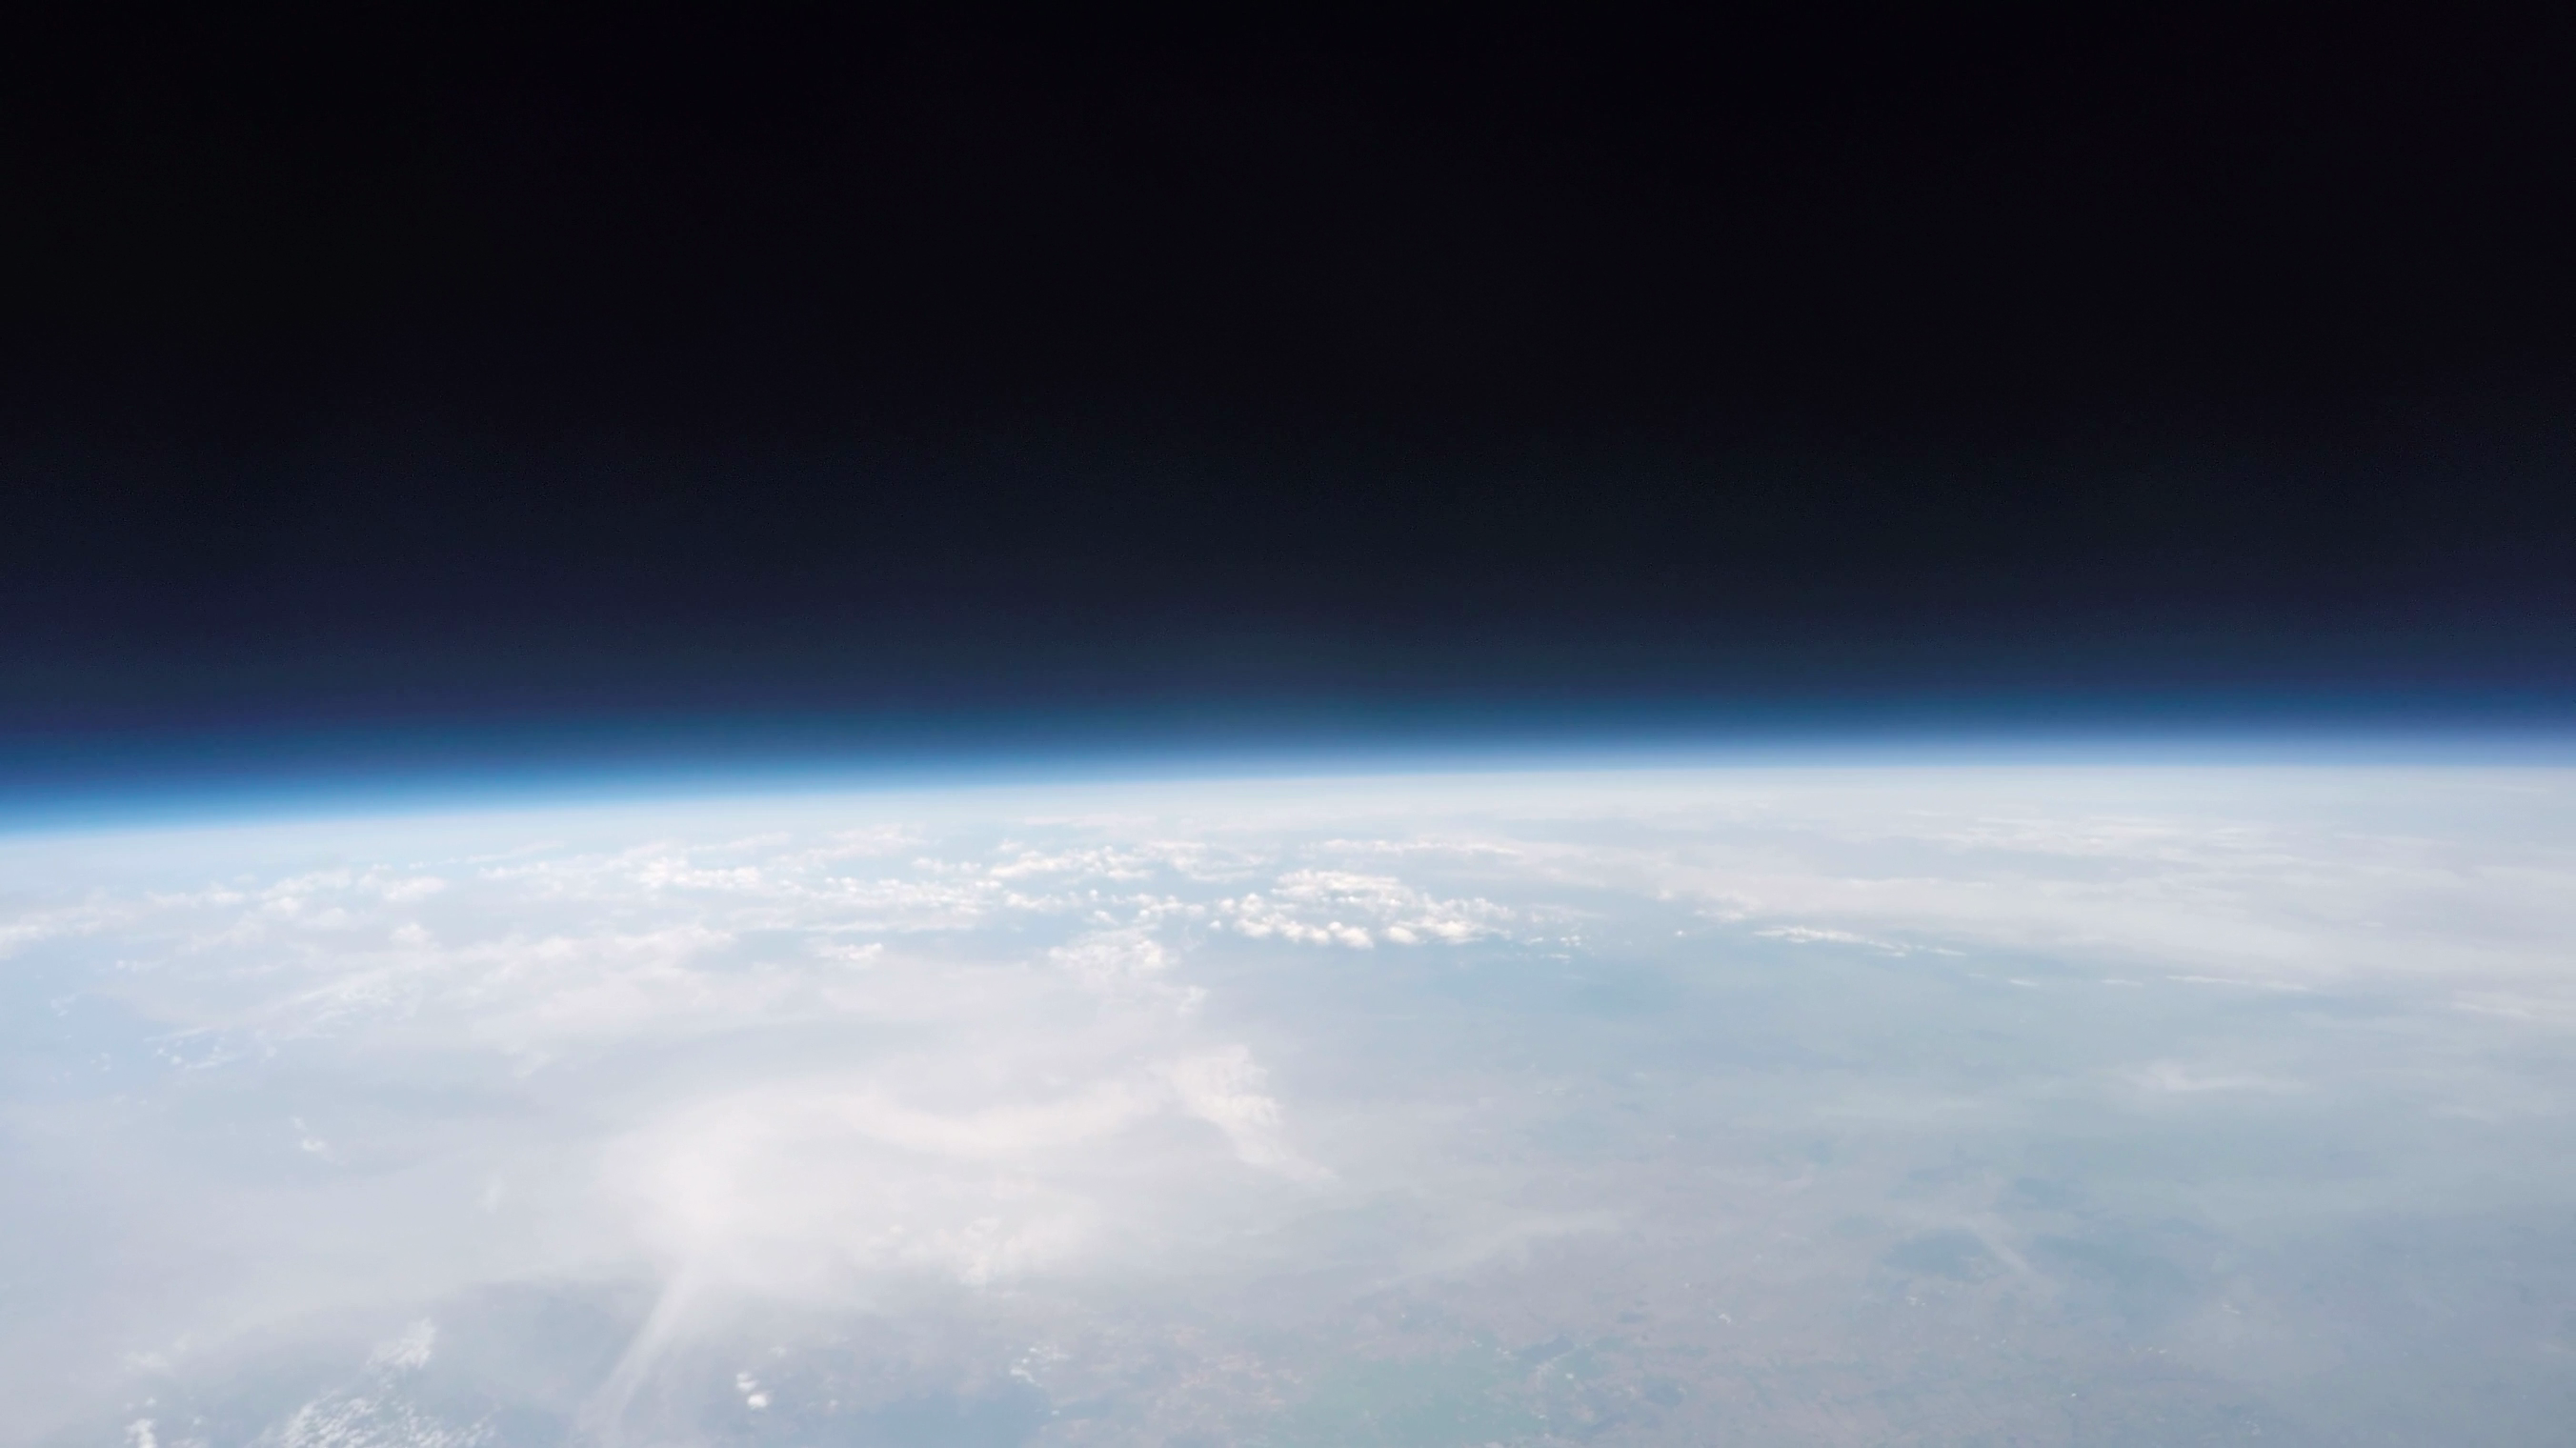
\includegraphics[scale=0.1]{test}
  \caption{this is a test picture}
  \label{fig:test}
\end{figure}

reference to the picture use figure \ref{fig:test} on page \pageref{fig:test}
\section{Callbacks}
\lipsum[4-6]
\section{Conclusion}
\lipsum[4-6]
\begin{thebibliography}{9}
  \bibitem{article} Author,Title \emph{Bookname}, Band and publication number,Page,Year.
  \bibitem{conferences} Author, TItle \emph{Conference Name}, Page, Year
  \bibitem{book} Author, \emph{Title}, Publisher, Year
\end{thebibliography}
\end{document}
references not counted toward the page limit (12 pages)
tips
- no singular pronouns (I)
-keywords write as cursive
- limited the use of footnotes
-examples
- every concept should have a example
- if possible use only one example
- use a example that is easy to understand

